\section{Framework description}
\label{sec:method}

In this section, the proposed artificial neural networks-evolutionary algorithm (\gls{ann-ea}) based method for prognostics is presented. Our method uses a multi-layer perceptron (\gls{mlp}) as the main regressor for estimating the \gls{rul} of the engines at each subset of the \gls{cmaps} dataset. For the training sets, the feature vectors are generated by using a strided time window while the labels vectors are generated using a constant \gls{rul} for the early cycles of the simulation and then linearly decreasing the number of remaining cycles, this is the so-called piecewise linear degradation model \citep{Ramasso2014}. For the test set, a time window is taken from the last sensors readings of the engine and used to predict the \gls{rul} of the engine.

The window-size $n_w$, window-stride $n_s$, and early-\gls{rul} $R_e$ data-related parameters, which for the sake of clarity and formalism in this study are considered as components of a vector $\nu \in \mathbb{Z}^3$ such that $\nu = (n_w, n_s, R_e)$, have a considerable impact on the quality of the predictions made by the regressor. Handpicking the best parameters, i.e. $\nu$,  is time consuming, furthermore, grid search approaches as the ones used for hyperparameter tuning in neural networks are computationally expensive given the dimension of the search spaces of the data-related parameters. In this paper, we propose the use of an evolutionary algorithm to fine tune the data-related parameters. The optimization framework here proposed allows for the use of a simple neural network architecture while attaining better results in terms of the quality of the predictions made by the other methods in the current literature.

\subsection{The Neural Network Architecture}

For this study we propose to use a rather simple \gls{mlp} architecture and the structure of the network remained consistent for all the four subsets. All the implementations were done in python using the Keras/Tensorflow environment, the source code is publicly available at the git repository \url{https://github.com/dlaredo/NASA_RUL_-CMAPS-}. 

The choice of the network architecture was made using an iterative process; comparing 6 different architectures, training each for $100$ iterations using a mini-batch size of $512$ and averaging their results over $10$ different runs. Two objectives were pursued: that the architecture was compact, e.g. in terms of layers and neurons within each layer, and that the performance indicators presented in Section \ref{sec:rul_dataset} were minimized. 

The process for choosing the network architecture is as follows: First, chose a fixed $\nu$, for the following experiment let $\nu = (30, 1, 140)$. Next, six different \gls{ann} architectures are defined, details of the architectures are provided in Appendix \ref{sec:appendices}. For each of the six different architectures, the performance is assessed using a cross-validation set from subset 1 of \gls{cmaps}. Table \ref{table:tested_architectures_100} summarizes the results for each tested architectures while Table \ref{table:proposed_nn} presents the architecture chosen for the remainder of this work. The chosen architecture provided the best compromise between compactness and performance among the rest of the tested architectures. 

\begin{table}[!htb]
\centering

\begin{tabular}{l | r r r r | r r r r}
	\hline	
	& \multicolumn{4}{| c}{RMSE} & \multicolumn{4}{| c}{RHS} \\
	Tested Architecture & Min. & Max. & Avg. & STD & Min. & Max. & Avg. & STD\\
  	\hline
  	Architecture 1 & 15.86 & 17.26 & 16.47 & 0.43 & 5.98 & 10.06 & 7.33 & 1.11\\
  	Architecture 2 & 15.56 & 17.15 & 16.35 & 0.65 & 6.52 & 20.11 & 4.50 & 4.50\\
  	Architecture 3 & 16.07 & 19.18 & 17.67 & 1.12 & 6.91 & 19.18 & 12.78 & 4.72\\
  	Architecture 4 & 15.32 & 19.99 & 17.63 & 1.48 & 5.93 & 24 & 13.54 & 6.28\\
  	Architecture 5 & 15.70 & 17.24 & 16.37 & 0.49 & 4.84 & 8.57 & 6.35 & 1.25\\
  	Architecture 6 & 15.58 & 16.92 & 15.95 & 0.39 & 5.44 & 7.65 & 6.38 & 0.68\\
  	\hline
\end{tabular}

\caption{Results for different architectures for subset 1, 100 epochs}
\label{table:tested_architectures_100}
\end{table}

\begin{table}[!htb]
\centering
\begin{tabular}{l l l l}
	\hline
	Layer & Shape & Activation & Additional Information\\
  	\hline
  	Hidden layer & 20 & ReLU & L2 regularization factor = 0.2\\
  	Output layer & 1 & Linear & \\
  	\hline
\end{tabular}
\caption{Proposed Neural Network architecture}
\label{table:proposed_nn}
\end{table}

\subsection{Shaping the data}

This section covers the data preprocessing applied to the raw sensors readings in each of the datasets. Although the original datasets contains $21$ different sensors readings, some of the sensors do not present much variance or convey redundant information, such sensors are therefore discarded. In the end, only $14$ sensors out of the $21$ are considered for this study, their indices in the \gls{cmaps} dataset are $\left\lbrace 2, 3, 4, 7, 8, 9, 11, 12, 13, 14, 15, 17, 20, 21 \right\rbrace$. The raw measurements are then used to create the strided time windows with window-size $n_w$ and window-stride $n_s$. For the training labels, $R_e$ is used at the early stages and then the \gls{rul} is linearly decreased. The data is also normalized to be within the range $\left[ -1,1 \right]$ using the min-max normalization.

\begin{equation}
\hat{x}_i = 2* \frac{x_i - min(x_i)}{max(x_i) - min(x_i)} - 1,
\label{eq:min_max_norm}
\end{equation}
where $x_i$ denotes the $m$-dimensional vector whose components are all the readings for the \textit{i-th} sensor and $\hat{x}_i$ is the normalized $x_i$ vector.

\subsubsection{Time Window Processing}

In multivariate time-series based problems such as \gls{rul}, more information can be generally obtained from the temporal sequence of data as compared with the multivariate data point at a single time stamp. Let $n_w$ denote the size of the time window, for a time window with a stride $n_s = 1$, all the past sensors values within the time window are collected and put together to form a feature vector $\mathbf{x}$. This approach has successfully been tested in \citep{Li2018, Lim2016} where the authors propose the use of a moving window with values raging from 20 to 30. In this paper we propose not only the use of a moving time window, but also a \textit{strided} time window that updates $n_s$ elements at the time instead of $1$. A graphical depiction of the strided time window is shown in Figure \ref{fig:time_window}.

\begin{figure}[!htb]
\centering

\includegraphics[width=0.9\textwidth]{../img/time_window.png}
\caption{Graphical depiction of the time window used in this framework.}
\label{fig:time_window}
\end{figure}

The use of a \textit{strided time window} allows for the regressor to take advantage not only of the previous information available, but also to control the ratio at which the algorithm is fed with new information. With the usual time window approach only one point is updated for every new time window, on the contrary, the strided time window allows for updating $n_s$ points at the time, allowing for the algorithm to catch newer information with fewer iterations, furthermore, the information contained in the strided time window is likely more rich than the one contained in a time window with stride of one.

\subsubsection{Piecewise linear degradation model}

Different from common regression problems, the desired output value of the input data is difficult to determine for a \gls{rul} problem. It is usually impossible to evaluate the precise health condition and estimate the \gls{rul} of the system at each time step without an accurate physics based model. For this kind of applicatios, a piece-wise linear degradation model has been proposed in \citep{Ramasso2014}. The piece-wise linear degradation model assumes that the engines have a constant \gls{rul} label in the early cycles and then the \gls{rul} starts degrading linearly until it reaches 0 as shown in Figure \ref{fig:piecewise_model}. The piecewise linear degradation approach is used for this work, in here we denote the value for the \gls{rul} at the early stages as $R_e$. 

\begin{figure}[!htb]
\centering
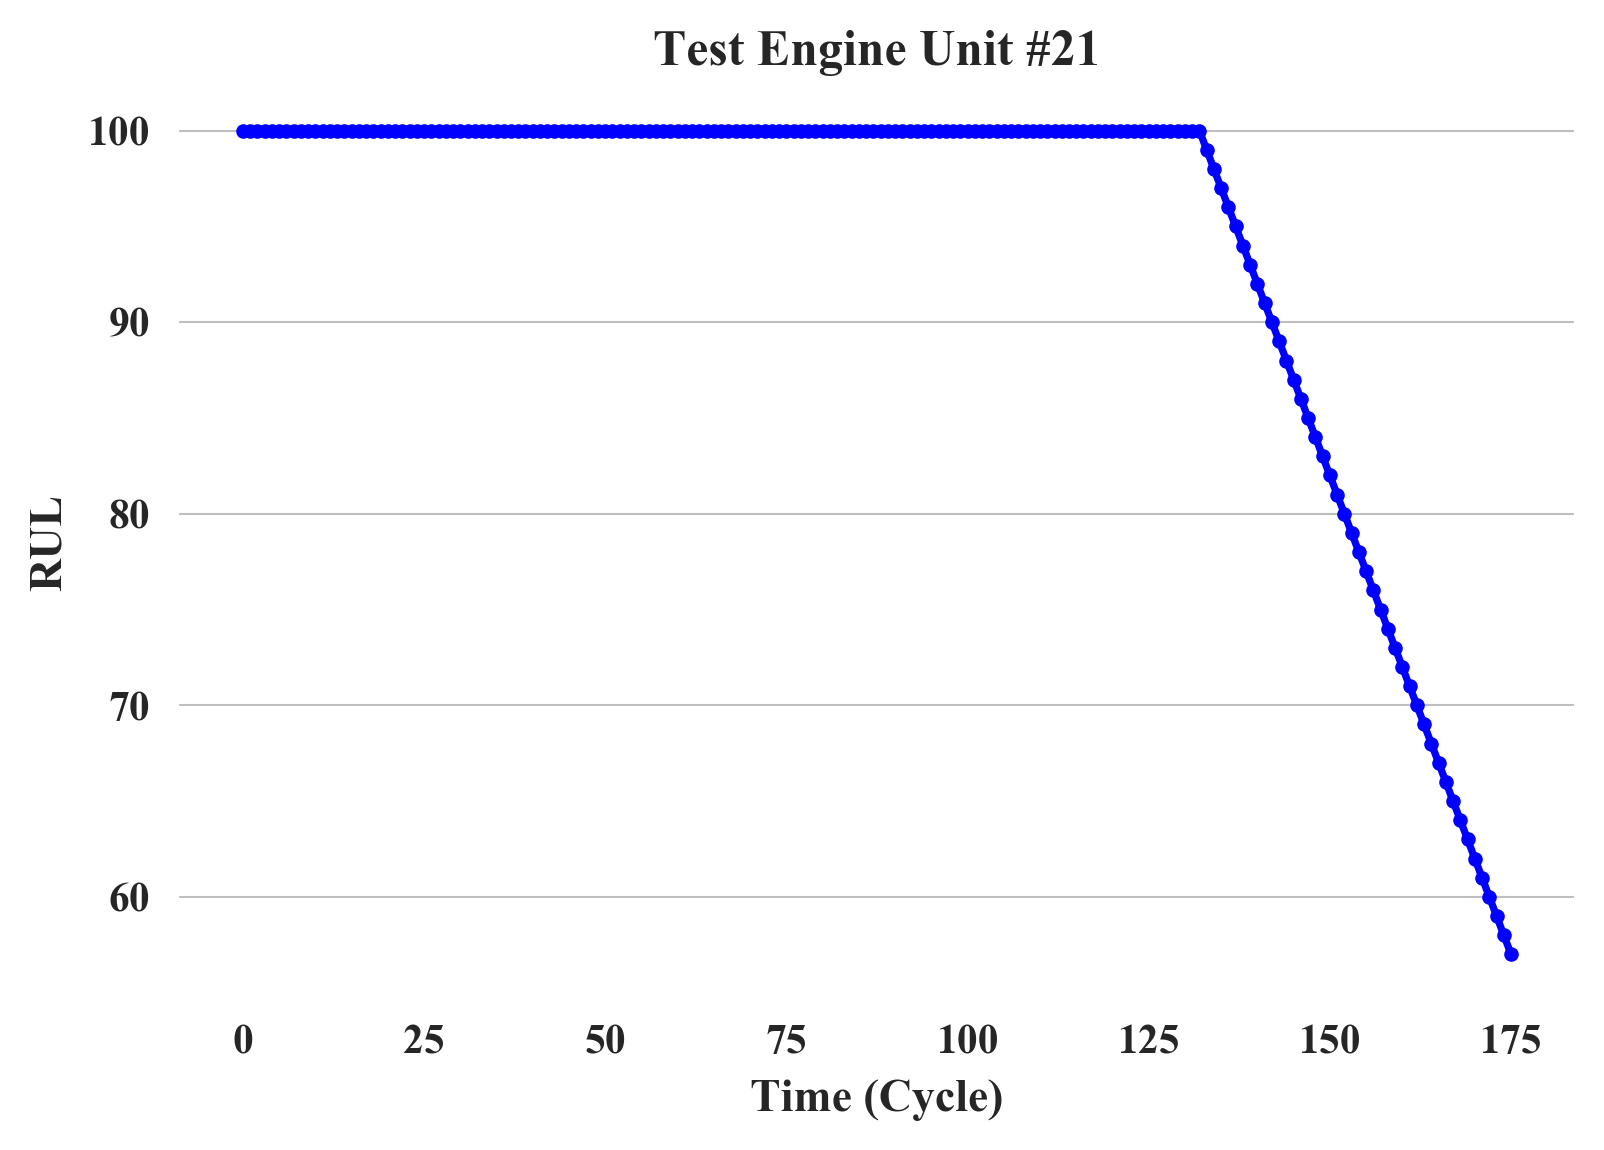
\includegraphics[width=0.7\textwidth]{../img/test_engine.png}
\caption{Piecewise linear degradation for \gls{rul}.}
\label{fig:piecewise_model}
\end{figure}

\subsection{Choosing optimal data-related parameters}
\label{sec:choosing_otimal_data-related_params}

As mentioned in the previous sections, the choice of the data-related parameters $\nu$ has a large impact on the performance of the regressor, i.e. the \gls{mlp}. In this section we present a framework for picking the optimal combination of the data-related parameters $n_w$, $n_s$ and $R_e$ while being computationally efficient.

Recall that $\nu = (n_w, n_s, R_e)$, where $n_w \in \left[1, b\right]$, $n_s \in \left[1, 10\right]$, and $R_e \in \left[90, 140 \right]$ are the specific boundaries for the \gls{cmaps} dataset and all the intervals are integer. The value of $b$ is dependent upon the specific subset, Table \ref{table:b_values} presents the different values $b$ can take for each dataset.

\begin{table}[!htb]
\centering
\begin{tabular}{l | l l l l}
	\hline
	 & FD001 & FD002 & FD003 & FD004\\
  	\hline
  	$b$ & 30 & 20 & 30 & 18\\
  	\hline
\end{tabular}
\caption{Allowed values for $b$ per subset}
\label{table:b_values}
\end{table}

Let also $X(\nu)$ be the training/cross-val/test sets parametrized by $\nu$ and used by the \gls{mlp} to perform the \gls{rul} estimation. Finally, let $f(\nu)=e_{rms}(X(\nu))$, recall from Equation (\ref{eq:rmse}) that $d = \hat{y} - y$ and that $\hat{y}$ depends on $X(\nu)$, also note that one function evaluation of $f(\nu)$ implies training the \gls{mlp} and computing the result of Equation (\ref{eq:rmse}). Here we propose to fine tune $\mathbf{\nu}$, formally speaking

\begin{equation}
\begin{aligned}
& \underset{\nu \in \mathbb{Z}^3}{\text{min}}
& & f(\nu) \\
\end{aligned}
\label{eq:optimization_problem}
\end{equation}

Given the nature of the problem at hand; namely that no analytical form of the problem is given, gradient information is unavailable, and the integer nature of the function variables, an evolutionary algorithm is the natural choice for the optimization process.

\subsubsection{Obtaining the true optimal data-related parameters}

The size of \gls{cmaps} dataset and the search space of $\nu$ allows for an exhaustive search to be performed in order to find the true optimal data-related parameters. We would like to emphasize tough, that although exhaustive search is a possibility for \gls{cmaps} dataset it is in no way a possibility in a more general setting, therefore the use of the evolutionary algorithm (\gls{ea}) adopted in this framework. Nevertheless, the possibility to perform exhaustive search on the \gls{cmaps} dataset can be exploited to demonstrate the accuracy of the chosen \gls{ea} and of the framework overall. Taking subsets FD001 and FD002 an exhaustive search is performed to find the true optimal values for $\nu$. The \gls{mlp} is trained for only $20$ epochs as in this experiment we are only interested in comparing the effect of different combinations for $\nu$ instead of obtaining the best performance. Table \ref{table:true_optimal_data_params} shows the optimal as well as the worst combinations of data-related parameters $\nu$ and the total number of function evaluations used by the exhaustive search.

\begin{table}[!htb]
\centering
\begin{tabular}{l | c r c r r l}
	\hline
	 Dataset & argmin $\nu$ & min $f(\nu)$ & argmax $\nu$ & max $f(\nu)$ & Function evals.\\
  	\hline
  	FD001 & $\left[ 30, 1, 125 \right]$ & $17.43$ & $\left[ 19, 1, 97 \right]$ & $80.92$ & 7500\\
  	FD002 & $\left[ 20, 1, 135 \right]$ & $36.89$ & $\left[ 19, 10, 109 \right]$ & $76.80$ & 2500\\
  	\hline
\end{tabular}
\caption{Exhaustive search results for subsets FD001 and F002.}
\label{table:true_optimal_data_params}
\end{table}

\subsubsection{Evolutionary algorithms for obtaining the optimal data-related parameters}
\label{sec:ea_optimization_process}

Evolutionary algorithms/meta-heuristics are a family of methods that optimize a problem by iteratively trying to improve a set of candidate solutions with regard to a given measure of quality. The methods do not make any assumptions about the problem, treating it as a black box that merely provides a measure of quality given a candidate solution. Furthermore \glspl{ea} do not require the gradient of the problem being optimized, making them very suitable for applications such as neural networks. Among the drawbacks of this kind of methods are that they usually require considerable computing effort to converge to a solution.

For this particular application, differential evolution (\gls{de}) \citep{Storn1997} is chosen as the optimization algorithm. Though in principle any meta-heuristic capable of handling integer variables is suitable for this application, \gls{de} has been stablished itself as one of the most reliable, robust and easy to use \glspl{ea}. Furthermore, a ready to use python implementation of \gls{de} is available through the scipy package \citep{scipy}. Although \gls{de} does not have special operators for treating integer variables a very simple modification to the algorithm, consisting on rounding every component of a candidate solution $\nu'$ to its nearest integer, is used for this work.

As mentioned earlier, evolutionary algorithms such as \gls{de} tend to use several function evaluations for obtaining the optimal solutions, recall that for this application one function evaluations implies retraining the  neural network from scratch. This is not a desirable scenario, as obtaining the optimal data-related parameters $\nu$ would entail an extensive use of computational power. Instead of running for \gls{de} for several iterations and with a large population size we propose to run it just for $30$ iterations (generations in the literature of evolutionary computation) and using a population size of $12$, which seems reasonable given the size of the search space of $\nu$. 

Furthermore, during the optimization process the \gls{mlp} is not trained for  $100$ epochs but for just $20$ instead, this is done mainly for two reasons: the use of the mini-batch in the training process allows for a speed up in the convergence, therefore it can be assumed that the algorithm will most likely be very close to its optima after just a couple of iterations, second and most important is the assumption that parameters that lead to lower score values in the early stages of the \gls{mlp} training process are more likely to provide better performance when trained for a larger number of epochs. Given the similarities between subsets FD001/FD003 and FD002/FD004 we have decided to just tune $\nu$ for subsets FD001 and FD002 and then use the obtained results on sets FD003 and FD004 respectively. Details for the use of \gls{de} in finding the optimum data-related parameters are described in Table \ref{table:de_hyperparams}.

\begin{table}[!htb]
\centering
\begin{tabular}{l l l l l}
	\hline
	 Population Size & Generations & Strategy & \gls{mlp} epochs\\
  	\hline
  	12 & 30 & Best1Bin & 20\\
  	\hline
\end{tabular}
\caption{Differential Evolution hyper-parameters.}
\label{table:de_hyperparams}
\end{table}

\begin{comment}
\begin{table}[!htb]
\centering
\begin{tabular}{l l l l l}
	\hline
	 Dataset & Window Size $n_w$ & Window Stride $n_s$ & Early RUL $R_e$\\
  	\hline
  	FD001 & 26 & 2 & 100\\
  	FD002 & 16 & 2 & 91\\
  	FD003 & 30 & 2 & 97\\
  	FD004 & 16 & 2 & 92\\
  	\hline
\end{tabular}
\caption{Optimal data-related parameters for each subset.}
\label{table:optimal_data_params}
\end{table}
\end{comment}

The optimal data-related parameters for each of the subsets found by \gls{de} are shown in Table \ref{table:optimal_data_params}. As can be observed the results obtained by \gls{de} are in fact very close to the real optima (displayed in Table \ref{table:true_optimal_data_params}) for both datasets, nevertheless the computational burden is reduced by one order of magnitude when using \gls{de}. From the results in Table \ref{table:optimal_data_params} it can be observed that the maximum allowable time window is always preferred while, on the contrary, small window strides yield better results, for the case of early RUL it can be observed that large $R_e$ improve the results.

\begin{table}[!htb]
\centering
\begin{tabular}{l | c r r l}
	\hline
	 Dataset & argmin $\nu$ & min $f(\nu)$ & Function evals.\\
  	\hline
  	FD001 & $\left[ 30, 1, 128 \right]$ & $17.78$ & 372\\
  	FD002 & $\left[ 20, 2, 134 \right]$ & $37.65$ & 372\\
  	\hline
\end{tabular}
\caption{Data-related parameters for each subset obtained with Differential Evolution.}
\label{table:optimal_data_params}
\end{table}

\subsection{The ANN-EA RUL estimation Framework}

Having described the major building blocks of the proposed method, we now introduce the complete framework in Algorithm \ref{alg:rul_framework}.

\setcounter{algorithm}{0}
\begin{algorithm}[H]
\caption{\gls{ann}-\gls{ea} \gls{rul} estimation Framework}\label{alg:rul_framework}
\textbf{Input:} Initial set of data-related parameters $\nu \in \mathbb{Z}^n$, Raw training/testing data $X$ and training labels $y$\\
\textbf{Output:} Optimal set of data-related parameters $\nu^*$
	\begin{algorithmic}[1]
		\State Choose regressor architecture (\gls{ann}, \gls{svm}, linear/logistic regression, etc).
		\State Define $f(\nu)$ as in Section\ref{sec:choosing_otimal_data-related_params}.
		\State Optimize $f(\nu)$ using the preferred evolutionary algorithm, i.e. differential evolution, evolutionary strategies, genetic algorithm, etc, using the proposed guidelines from Section \ref{sec:ea_optimization_process}.
		\State Use $\nu^*$ to train the regressor for as many epochs as needed.
	\end{algorithmic}
\end{algorithm}